\chapter{Revisão teórica}
\label{ch:revisão}

As definições utilizadas neste projeto foram, em grande parte,
retiradas de \cite{diestel2025graph}, com algumas modificações. Como
a implementação dos algoritmos está em inglês, também apresentaremos
o correspondente de cada definição em inglês, entre parênteses.

\begin{mydef}[Grafo]
  Um \emph{grafo} (\textit{graph}) é uma estrutura $G := (V, A)$
  tal que $A \subseteq V^2$ e $V$ é um conjunto de um tipo qualquer.
  Os elementos de $V$ são denominados vértices (\textit{nodes}) e os
  elementos de $A$ são denominados de arestas
  (\textit{edges}). O jeito tradicional de visualizar um
  grafo é como uma figura composta de bolas e setas:
  \begin{figure}[h]
    \centering
    \begin{tikzpicture}
      \GraphInit[vstyle=normal]
      \tikzset{EdgeStyle/.style={->}}
      \Vertices{circle}{1,2,3,4}
      \Edges(1,2,3)
      \Edge(1)(4)
    \end{tikzpicture}
    \caption{Um grafo com $V := \{1,2,3,4\}$ e $A :=
    \{(1,2),(1,4),(2,3)\}.$}
    \label{fig:graph1}
  \end{figure}
  \FloatBarrier
\end{mydef}

\begin{mydef}[Ordem e Tamanho]
  O número de vértices de um grafo $G$ é chamado de \emph{ordem}
  (\textit{order}) e é denotado por $|G|$ -- o número de arestas é chamado de
  \emph{tamanho} (\textit{size}) e é denotado por $||G||$. Por exemplo, na
  Figura~\ref{fig:graph1}, $|G| = 4$ e $||G|| = 3$.
\end{mydef}

\begin{mydef}[Adjacência]
  Dizemos que um vértice $v$ é \emph{adjacente}, ou \emph{vizinho},
  de um vértice
  $u$ (\textit{neighbor}) se somente se $(u,v) \in A$, também,
  denotaremos $(u,v)$ como $uv$. Visualmente,
  enxergamos isso como:
  \begin{figure}[h]
    \centering
    \begin{tikzpicture}
      \GraphInit[vstyle=normal]
      \tikzset{EdgeStyle/.style={->}}
      \Vertices{circle}{v,u}
      \Edge(u)(v)
    \end{tikzpicture}
    \caption{Um grafo com $V := \{u,v\}$ e $A :=
    \{(u,v)\}.$}
  \end{figure}
  \FloatBarrier
\end{mydef}

\begin{mydef}[Conjunto de adjacentes]
  Num grafo $G$, o conjunto de todos os vértices adjacentes de $u$
  (\textit{neighbors}) é denotado por $A_G(u) := \{v \in V\, |\, uv \in
  A\}$. Já o conjunto de todos os vértices que em que $v$ é adjacente
  será denotado por $\bar{A}_G(u) := \{ v \in V\, |\, vu \in A\}$.
\end{mydef}

\begin{mydef}[Grau de um vértice]
  O \emph{grau de um vértice} $v$ (\textit{node degree}) é o valor
  correspondente da soma $|A_G(v)| + |\bar{A}_G(v)|$. Também
  denotamos $|A_G(v)|$ como $d^+(v)$, $|\bar{A}_G(v)|$ como $d^-(v)$ e
  sua soma como $d(v)$.
\end{mydef}

\begin{mydef}[Caminho]
  Um \emph{caminho} (\textit{path}) é um grafo $C := (V, A)$ que tem a forma:
  \begin{displaymath}
    V := \{x_0, x_1,...,x_k\} \qquad A := \{x_0x_1,x_1x_2,...,x_{k-1}x_k\}
  \end{displaymath}
  Dizemos que $C$ é um caminho de $x_0$ a $x_k$. Normalmente nos
  referimos ao caminho como a sequência dos seus vértices, $x_0x_1...x_k$.
\end{mydef}

\begin{mydef}[Conectividade]
  Dizemos que um grafo $G$ é conexo (\textit{connected}) se somente
  se para quaisquer dois vértices $u$ e $v$, existe um caminho entre eles.
\end{mydef}

\begin{mydef}[Grafo não direcionado]
  Dizemos que um grafo $G$ é \emph{não direcionado}
  (\textit{undirected}) se somente se $A$ é simétrico, ou seja, se
  $uv \in A$ então $vu \in A$. O nome não direcionado vem da ideia de
  que os grafos que viemos discutindo até agora são denomidados de
  \emph{direcionados}, ou simplesmente \emph{dígrafos}. Na
  literatura é comum apresentar grafo não direcionado como grafo e
  depois o direcionado como dígrafo, resolvemos inverter a ordem pois
  assim se traduz melhor nas representações de grafos que vamos
  implementar. Um grafo não direcionado pode ser visualizado sem a
  ponta das setas:

  \begin{figure}[h]
    \centering
    \begin{tikzpicture}
      \GraphInit[vstyle=normal]
      \Vertices{circle}{c,b,a}
      \Edges(a,b,c)
    \end{tikzpicture}
    \caption{Um grafo não direcionado com $V := \{a,b,c\}$ e $A :=
    \{ab,ba,bc,cb\}$}
    \label{fig:ungraph1}
  \end{figure}

  Também é comum omitir a simetria das arestas se pelo contexto for
  claro que está sendo tratado de um grafo não direcionado, na
  Figura~\ref{fig:ungraph1}, o conjunto de arestas $A$ seria escrito
  como $\{ab,bc\}$.
\end{mydef}

\begin{mydef}[Grafo subjacente]
  O grafo subjacente (\textit{underlying}) de um grafo direcionado $G
  := (V, A)$ é o grafo $S := (V, A')$ onde $A' := \{vu\, |\, uv \in A\} \cup A$.
\end{mydef}

\begin{mydef}[Grafo Bipartido]
  Dizemos que um grafo $G := (V, A)$ é bipartido (\textit{bipartite})
  se somente se existem dois conjuntos disjuntos $V_1$, $V_2$ tal que
  $V_1 \cup V_2 = V$, e que para todo $(u, v) \in A$, ($u \in
  V_1$ e $v \in V_2$) ou ($u \in V_2$ e $v \in V_1$), isto é, toda
  aresta em $A$ conecta um vértice de $V_1$ a um vértice de $V_2$.
  \begin{figure}[h]
    \centering
    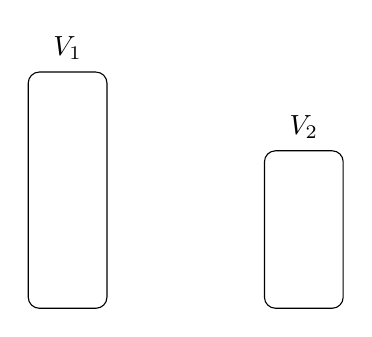
\begin{tikzpicture}
      \GraphInit[vstyle=normal]
      \SetGraphUnit{2}

      % V_1
      \Vertex[x=0,y=3]{a}
      \Vertex[x=0,y=2]{b}
      \Vertex[x=0,y=1]{c}

      % V_2
      \Vertex[x=3,y=2]{u}
      \Vertex[x=3,y=1]{v}

      % Bipartite edges
      \Edge(a)(u)
      \Edge(b)(v)
      \Edge(b)(u)
      \Edge(c)(v)

      % Partitions
      \draw[rounded corners] (-0.5, 0.5) rectangle (0.5, 3.5);
      \node at (0, 3.8) {$V_1$};
      \draw[rounded corners] (2.5, 0.5) rectangle (3.5, 2.5);
      \node at (3, 2.8) {$V_2$};
    \end{tikzpicture}
    \caption{Um grafo bipartido com $V_1 := \{a,b,c\}$ e $V_2 := \{u,v\}$}
  \end{figure}
  \FloatBarrier
\end{mydef}

\begin{mydef}[Grafo Biconexo]
  Dizemos que um grafo $G := (V, A)$ é biconexo
  (\textit{biconnected}) se somente se $|G| > 2$ e para todo $v \in
  V$,  o subgrafo de $G$ resultante da remoção de $v$ é conexo, isto
  é, $G - \{v\}$ é conexo.
\end{mydef}
